
\newcommand{\prophetmax}{%
\begin{figure}[h!]\label{fig:random}
	\centering
	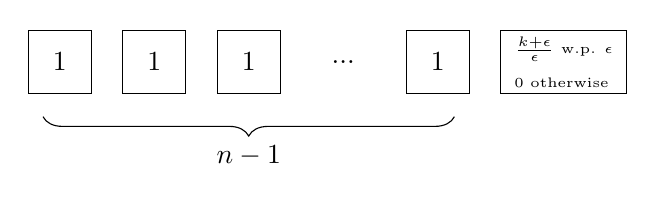
\begin{tikzpicture}[scale=0.4]
		\draw (0,0) rectangle node (C) {$1$} ++(2,2); 
		\draw (3,0) rectangle node (D) {$1$} ++(2,2); 
		%\draw (6,0) rectangle node (E) {$1$} ++(2,2); 
		\draw (6,0) rectangle node (F) {$1$} ++(2,2); 
		\draw [draw=white](9,0) rectangle node (dots) {...} ++(2,2); 
		\draw (12,0) rectangle node (A) {$1$} ++(2,2); 
		\draw (15,0) rectangle node (B)[align=left] {\tiny$\frac{k+\epsilon}{\epsilon}$ w.p. $\epsilon$\\\tiny$0$ otherwise} ++(4,2); 
		\draw[decorate,decoration={brace, amplitude=7pt, raise=13pt, mirror}]
		(C.south west) to node[black,below= 20pt] {$n-1$} (A.south east);%
	\end{tikzpicture}
	\caption{An example where the expected reward is no more than $\frac{1}{k+\ell}\sum_{j=1}^{\ell} \E [y_j]+\epsilon$}
	
\end{figure}
}


\newcommand{\prophetpoa}{%

\begin{figure}
	\centering
	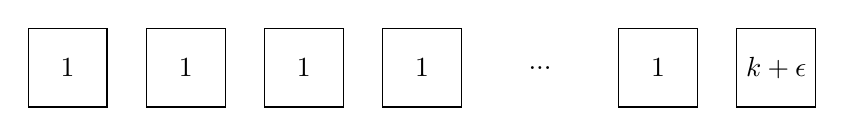
\begin{tikzpicture}[scale=0.5]
	\draw (0,0) rectangle node (A) {$1$} ++(2,2); 
	\draw (3,0) rectangle node (B) {$1$} ++(2,2); 
	\draw (6,0) rectangle node (C) {$1$} ++(2,2); 
	\draw (9,0) rectangle node (D) {$1$} ++(2,2); 
	\draw [draw=white](12,0) rectangle node (dots) {...} ++(2,2); 
	\draw (15,0) rectangle node (E) {$1$} ++(2,2); 
	\draw (18,0) rectangle node (F) {$k+\epsilon$} ++(2,2); 
	\end{tikzpicture}
	\caption{An example where the price of anarchy is $2$}
\end{figure}
		
}
\newcommand{\prophetlexlong}{%
	
\begin{figure}[h!]\label{fig:ranked}
	\centering
	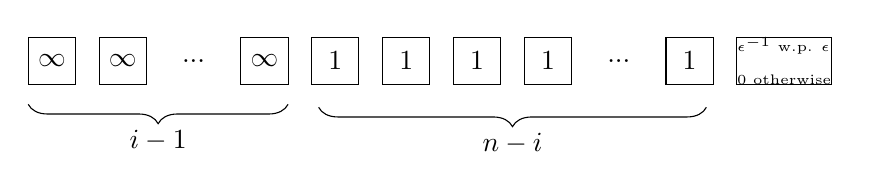
\begin{tikzpicture}[scale=0.3]
	\draw (0,0) rectangle node (G) {$\infty$} ++(2,2); 
	\draw (3,0) rectangle node (H) {$\infty$} ++(2,2); 
	\draw [draw=white](6,0) rectangle node (dots) {...} ++(2,2); 
	\draw (9,0) rectangle node (J) {$\infty$} ++(2,2); 
	\draw (12,0) rectangle node (C) {$1$} ++(2,2); 
	\draw (15,0) rectangle node (D) {$1$} ++(2,2); 
	\draw (18,0) rectangle node (E) {$1$} ++(2,2); 
	\draw (21,0) rectangle node (F) {$1$} ++(2,2); 
	\draw [draw=white](24,0) rectangle node (dots) {...} ++(2,2); 
	\draw (27,0) rectangle node (A) {$1$} ++(2,2); 
	\draw (30,0) rectangle node (B)[align=left] {\tiny${\epsilon}^{-1}$ w.p. $\epsilon$\\\tiny$0$ otherwise} ++(4,2); 
	\draw[decorate,decoration={brace, amplitude=7pt, raise=10pt, mirror}]
	(C.south west) to node[black,below= 16pt] {$n-i$} (A.south east);%
	\draw[decorate,decoration={brace, amplitude=7pt, raise=10pt, mirror}]
	(G.south west) to node[black,below= 16pt] {$i-1$} (J.south east);%
	\end{tikzpicture}
	\caption{An example where the expected reward for agent $i$ is no more than $\frac{1}{\ell+2}\sum_{j=i}^{i+\ell} \E [y_j]+\epsilon$}
	
\end{figure}
	
}


\newcommand{\prophetlex}{%
	
	\begin{figure}
		\centering
		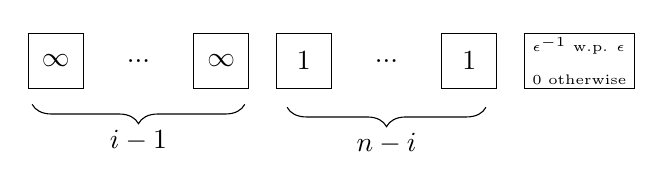
\begin{tikzpicture}[scale=0.35]
		\draw (0,0) rectangle node (G) {$\infty$} ++(2,2); 
		\draw [draw=white](3,0) rectangle node (dots) {...} ++(2,2); 
		\draw (6,0) rectangle node (J) {$\infty$} ++(2,2); 
		\draw (9,0) rectangle node (C) {$1$} ++(2,2); 
		\draw [draw=white](12,0) rectangle node (dots) {...} ++(2,2); 
		\draw (15,0) rectangle node (A) {$1$} ++(2,2); 
		\draw (18,0) rectangle node (B)[align=left] {\tiny${\epsilon}^{-1}$ w.p. $\epsilon$\\\tiny$0$ otherwise} ++(4,2); 
		\draw[decorate,decoration={brace, amplitude=7pt, raise=10pt, mirror}]
		(C.south west) to node[black,below= 16pt] {$n-i$} (A.south east);%
		\draw[decorate,decoration={brace, amplitude=7pt, raise=10pt, mirror}]
		(G.south west) to node[black,below= 16pt] {$i-1$} (J.south east);%
		\end{tikzpicture}
		\caption{An example where the expected reward for agent $i$ is no more than $\frac{1}{\ell+2}\sum_{j=i}^{i+\ell} \E [y_j]+\epsilon$}
		
	\end{figure}
	
}